% JuliaCon proceedings template
\documentclass{juliacon}
\setcounter{page}{1}
\usepackage{amsmath}
\usepackage{cleveref}
\usepackage{microtype}

%% extra links:
%% - GPU Julia: https://cuda.juliagpu.org/stable/tutorials/introduction/
%% - GPU x2: https://nextjournal.com/sdanisch/julia-gpu-programming
%% - NaN vs missing https://discourse.julialang.org/t/is-there-any-reason-to-use-nan-instead-of-missing/84396

\begin{document}

% Misc typographical tweaks.
\setlength{\parindent}{1.2em}
% \setmonofont{JuliaMono}[Extension = .ttf, Path = ./, UprightFont = *-Regular, ItalicFont = *-Italic]

% **************GENERATED FILE, DO NOT EDIT**************

\title{My JuliaCon proceeding}

\author[1]{Taylor Allred}
\author[1]{Xinyi Li}
\author[1]{Ashton Wiersdorf}
\author[1]{Ben Greenman}
\author[1]{Ganesh Gopalakrishnan}
\affil[1]{University of Utah}

\keywords{Julia, Optimization, Game theory, Compiler}

\hypersetup{
pdftitle = {My JuliaCon proceeding},
pdfsubject = {JuliaCon 2019 Proceedings},
pdfauthor = {1st author, 2nd author, 3rd author},
pdfkeywords = {Julia, Optimization, Game theory, Compiler},
}


\maketitle

\begin{abstract}
  Reliable numerical computations are central to high-performance computing and machine learning.
  However, floating-point numbers exhibit non-intuitive behaviors that make writing correct numerical computation difficult.
  In particular, \emph{floating-point exceptions} occur when no mathematically sensible result is available, and it is difficult to find \emph{where} these exceptions occur.
  Unhandled exceptions can cause programs crash, exhibit bad behavior, or worse, silently produce good-looking but incorrect data.
  We present FlowFPX: a tool set for debugging floating-point code.
  FlowFPX can track floating-point exceptions occurring in Julia code to their sources.
  FlowFPX also detects otherwise silent exceptions which can foul program outputs.
  FlowFPX produces intuitive visualizations of summarized exception flows including how they are generated, propagated and killed, thus helping with debugging.
\end{abstract}

\newcommand{\code}[1]{\texttt{#1}}
\newcommand{\FlowFPX}{FlowFPX}
\newcommand{\GPUFPX}{GPU-FPX}
\newcommand{\FloatTracker}{FloatTracker}
\newcommand{\FT}{\FloatTracker}
\newcommand{\Fp}{Floating-point} % hyphen or no?
\newcommand{\fp}{floating-point} % hyphen or no?
\newcommand{\CSTG}{stack graph}
\newcommand{\CPP}{\code{C++}}
\newcommand{\Dendro}{\textsc{Dendro}}
\newcommand{\urlaccess}[2]{\url{#1}}
\newcommand{\Nan}{\code{NaN}}
\newcommand{\NaN}{\Nan}
\newcommand{\Inf}{\code{Inf}}
\newcommand{\zerowidth}[1]{\makebox[0pt][l]{#1}}
\newcommand{\zerocode}[1]{\zerowidth{\code{#1}}}

\section{Introduction}

Reliable numeric computations are central to high-performance computing,
machine learning, and scientific applications.
Yet, the \fp{} arithmetic that powers these computations is fundamentally
unreliable~(\cref{s:background}).
Exceptional values, such as Not a Number (\Nan{}) and infinity (\Inf{}),
can and often do arise thanks to culprits such as roundoff error,
catastrophic cancellation, singular matrices, and vanishing
derivatives~\cite{sdjmrstp-pc-2022,ddghlllprr-correctness-2022,gllprt-correctness-2021,fpchecker-reports,llg-soap-2022,bllmg-xloop-2022}.
When exceptions happen, domain experts must take time away from their main
focus and trek down a rabbit hole to find the source of the error.
There is little tool support to assist in this difficult task,
thus (unsurprisingly) a quick GitHub search reports over 4,000 open issues
related to \NaN{} or \Inf{} exceptions~\cite{github-issues}.

We introduce \FlowFPX{}, a toolkit for debugging
\fp{} exceptions~(\cref{s:flowfpx}):
\begin{itemize}
  \item
    The centerpiece of \FlowFPX{} is \FT{}, a dynamic analysis tool that uses
    Julia's operator overloading to selectively monitor for exceptions and to
    fuzz code for vulnerabilities.
  \item
    To visualize results, \FT{} adapts coalesced stack-trace graphs 
    (CSTGs, or \CSTG{}s)~\cite{humphreySystematicDebuggingMethods2014} for a whole-program view on the generation,
    propagation, and death of exceptional values.
  \item A companion tool \GPUFPX{}~\cite{llsflg-hpdc-2023} provides fine-grained insights for GPU kernels.
\end{itemize}
%
\FlowFPX{} has helped debug exceptions in a variety
of applications: from ocean simulations to heat models~(\cref{s:casestudies}).
This paper concludes with related work~(\cref{s:related}) and a
brief discussion~(\cref{s:discussion}).

\section{Floating-Point Exception Primer}
\label{s:background}

\Fp{} is essentially scientific notation---\fp{} numbers are represented by packing a sign bit, an exponent, and a fraction part (also called the ``significand'' or ``mantissa'') into contiguous bit fields.
The advantages of this representation are that allows for compact representation of both very small and very large numbers in a narrow range of bits---a 64-bit float can represent numbers as big as $2^{1024}$ and as small as $2^{-1074}$.
This range is sufficient to represent numbers as small as Planck's constant or as big as Avogadro's constant with reasonable accuracy.

\begin{figure}[h]
  \label{fig:real_vs_float}
  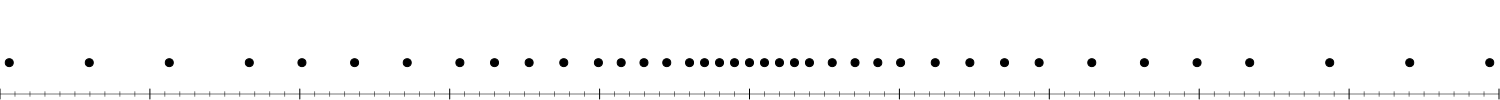
\includegraphics[width=\columnwidth]{ fig/real_vs_fp.png }
  \caption{The real number line vs the points representable with \fp{}.}
\end{figure}

The flip side is that not every real number within that wide range is representable as a \fp{} value---there is almost always some gap between the real number that we wish to represent and the \fp{} number that approximates that value.
Whenever a value we have doesn't have a precise representation, we must \emph{round} that real value to the nearest \fp{} value, which introduces some error in our calculations.
In addition to this error, the finite nature of \fp{} values means that we can run into some situations that wouldn't arise when working with real numbers.

For example, if two numbers' exponents differ by too large an amount, adding or subtracting the smaller from the bigger will leave us with just the bigger number.
Below we take the Planck constant and add it to Avogadro's constant and are left bit-for-bit with Avogadro's constant, as if we had never done any addition at all: there is no way to pack all the significant figures from true value that differs minutely from Avogadro's number into a 64-bit \fp{} number.

\begin{lstlisting}[language = Julia]
p = 6.62607015e-34
a = 6.02214076e23

println("planck:   $p : $(bitstring(p))")
println("avogadro: $a  : $(bitstring(a))")
println("p + a:    $(p + a)  : $(bitstring(p + a))")
\end{lstlisting}

You can see in the output that \texttt{p + a} is bit-for-bit equivalent to \texttt{a}:

\begin{lstlisting}
planck:   6.62607015e-34 : 0011100100001 ... 001
avogadro: 6.02214076e23  : 0100010011011 ... 111
p + a:    6.02214076e23  : 0100010011011 ... 111
\end{lstlisting}

This is a fairly extreme example; even when the numbers are closer in magnitude, most operations on \fp{} numbers induce loss of accuracy.

\subsection{Floating-Point Standards}

Prior to 1985, incomparable techniques for representing \fp{} values proliferated as mainframes and later personal computers emerged.
This made writing portable \fp{} code challenging.~\cite{houghIEEEStandard7542019}
IEEE 754~\cite{IEEEStandardBinary1985} standardizes \fp{} representation and operations across different architectures---these days, most machines and languages follow the IEEE 754 standard, and we make no effort to generalize our work beyond what IEEE 754 specifies.

\subsection{Exceptions and Exceptional Values}

IEEE 754 defines \emph{\fp{} exceptions}, which are events that occur when something goes wrong in a calculation.
William Kahan says,

\begin{quote}
An arithmetic exception arises when [there is] no result that would be acceptable universally.
\end{quote}

For example, dividing by zero is an exception, as is exceeding a \fp{} format's range.
These are exceptions because it is impossible to say what the right answer \emph{should} have been: perhaps that zero was meant to be a value that got really \emph{close} to zero,\footnote{The third kind of exceptional value is called a \emph{subnormal} value.} and suddenly rounded towards zero before division.
Or maybe that value that got really big \emph{does} need to get that big, but you need to start using a larger bit width for your \fp{} values.
Whatever, the case, there isn't a universally acceptable answer, so a \fp{} exception gets raised.

IEEE 754 doesn't force the programmer to always handle these exceptions, however, so we end up with \emph{exceptional values}, which are the results of exception-raising operations.
The two values we work with in this paper are \Inf{}\footnote{There are actually two infinities: $+\infty$ and $-\infty$; they behave the same for our purposes, so we will refer to them just as ``\Inf{}''.} and \NaN{}, which result from overflow and nonsensical operations respectively.
\Cref{fig:nan-gens} lists some of the situations that lead to exceptional values.

\begin{figure}[ht]
  \centering
  \label{fig:nan-gens}
  % \begin{tabular}{c | p{0.5 \columnwidth}}
  \begin{tabular}{c | c}
    \NaN{} & \Inf{} \\
    \hline
    $\tfrac{0}{0}$ & $\tfrac{x}{0},\, x \neq 0$ \\
    $0 * \infty$ & $\log{(0)}$ \\
    $\text{\texttt{NaN}} + x$ & $\infty + x,\, x \neq \text{\texttt{NaN}}$ \\
    $\infty - \infty$ & Any result exceeding \\
    & representation capacity
  \end{tabular}
  \caption{Examples of operations leading to exceptional values}
\end{figure}

For more details on exceptional values, see~\cite{knuthArtComputerProgramming1997,torontoPracticallyAccurateFloatingPoint2014} as well as the \textit{Handbook of Floating-Point Arithmetic}.~\cite{mullerHandbookFloatingPointArithmetic2018}

\subsection{Lifetimes of Unhandled Exceptions}
\label{s:to-kill-a-fp}

Exceptional values have a life cycle: instead a program-halting exception, an exceptional value comes into being at the point of an undefined operation and propagates through the rest of the computation.
Often they go on to manifest in the output of the code, but sometimes they can ``die'' by disappearing silently.
We characterize this life cycle in \cref{fig:gpk}.

\begin{figure}[ht]
  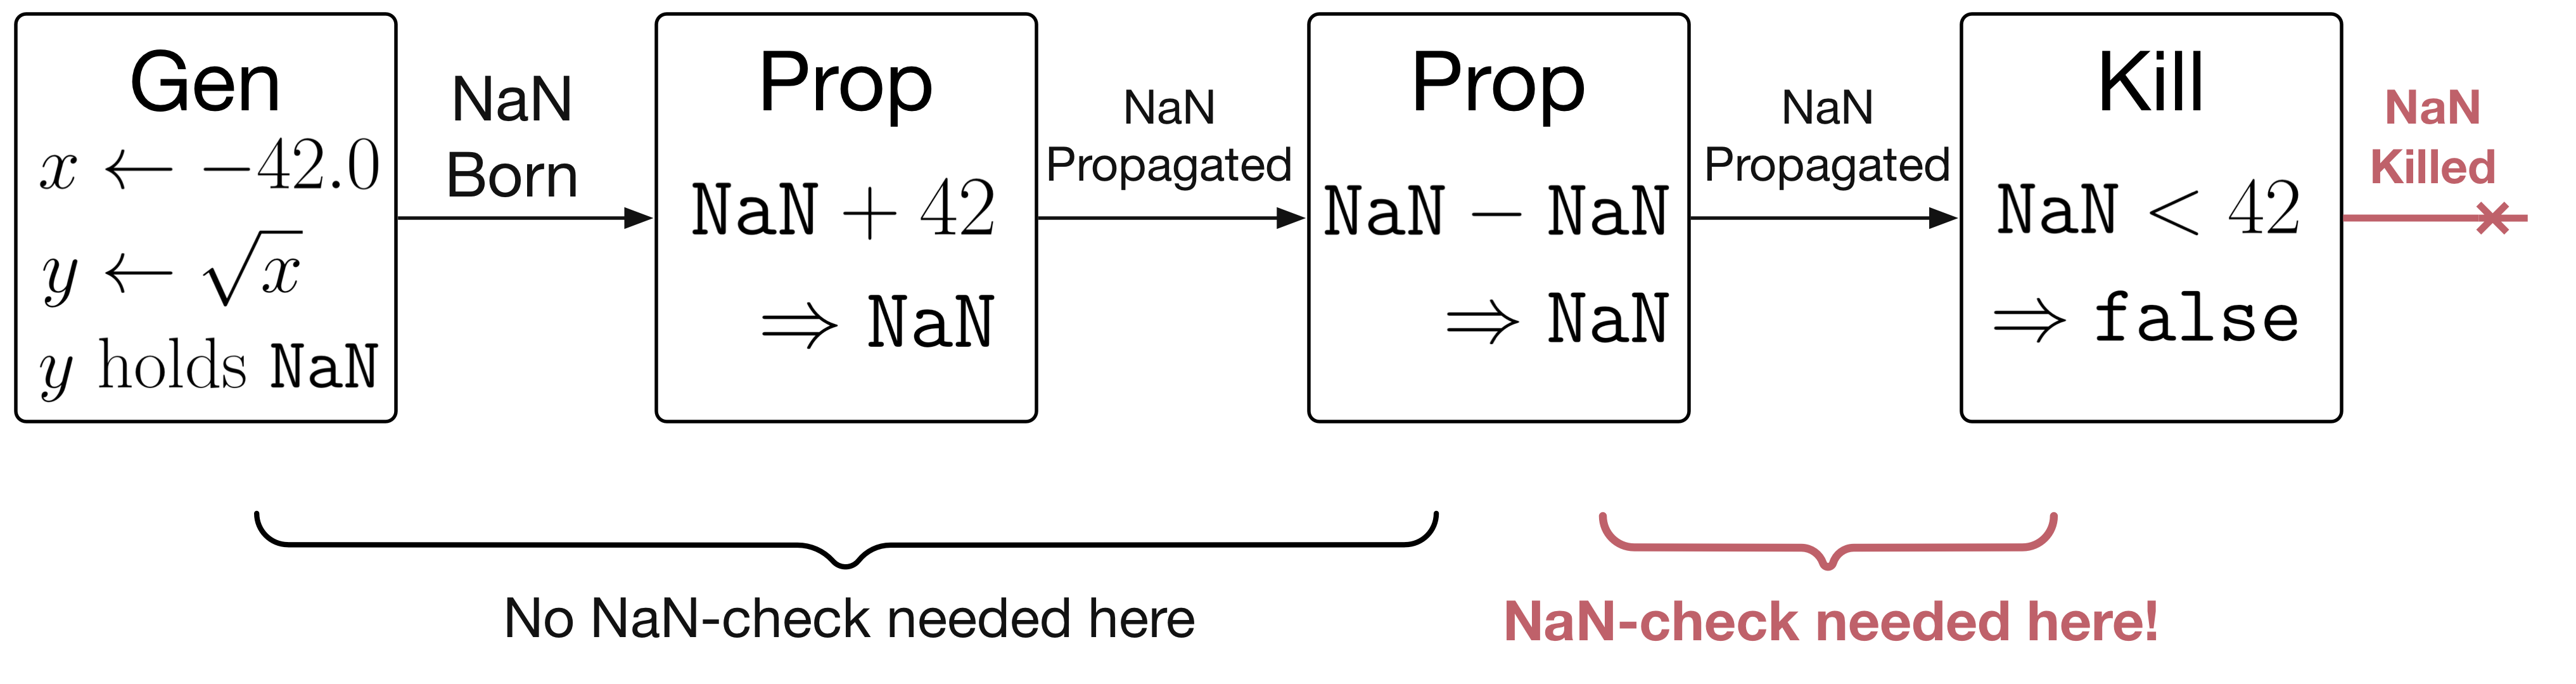
\includegraphics[width=\columnwidth]{fig/genpropkill-outline.png}
  \caption{Gen, Prop, Kill: Lifetime of a \NaN{} value}
  \label{f:gpk}
\end{figure}

When a \NaN{} or an \Inf{} comes into being as the result of an undefined operation, we call this a generation, or \emph{gen} for short.

Most of the time, when any or all of the arguments are \NaN{}, the result is also a \NaN{}.
We call this a propagation, or \emph{prop} for short.
This is good and desirable, because it means that an arithmetic error---even if buried deep in an expression---will still be observable, allowing a user to find and debug it.

However, there are a few places where exceptional values flow into an expression, but not out.
We call these instances \emph{kills}, and these can lead to subtle logic bugs.
For example, \emph{any} comparison ($<$, $>$, $=$, $\neq$, etc.) with a \NaN{} returns \texttt{false}.

Consider the following two functions to find the maximum value in a list:

\begin{lstlisting}[language = Julia]
function bad_max(lst)
  max_seen = 0.0
  for x in lst
    if ! (x <= max_seen)
      # swap if new val greater
      max_seen = x
    end
  end
  max_seen
end

function good_max(lst)
  foldl(max, lst)
end
\end{lstlisting}

Both \texttt{bad\_max} and \texttt{good\_max} compute the maximum in a list.
However, the \texttt{<=} operator used in the \texttt{bad\_max} implementation does \emph{not} propagate \NaN{}s: \texttt{NaN <= 4} returns \texttt{false}, not \NaN{}.
Because of this, you might not get the result you expected:

\begin{lstlisting}[language = Julia]
bad_max([1, 5, NaN, 4])     # returns 4
good_max([1, 5, NaN, 4])    # returns NaN
\end{lstlisting}

Not only is the result from \texttt{bad\_max} problematic for obscuring the fact that there was a \NaN{} in the list, the result is also wrong!
The built-in \texttt{max} function correctly propagates \NaN{}s, so we can see from its return that we got a \NaN{} somewhere.
It's not entirely obvious \emph{where} that \NaN{} came from.

\section{\FlowFPX{}}
\label{s:flowfpx}

\FlowFPX{} is a set of tools to aid in tracking down \fp{} exceptions.
The two primary tools we cover in this paper are \FT{} and CSTG:

\begin{itemize}
\item \FT{} traces the lifetime of exceptional \fp{} values and enables inside-out fuzzing.
\item CSTG visualizes the tracing output from \FT{} in compact form.
\end{itemize}

\GPUFPX~\cite{llsflg-hpdc-2023} is another component of \FlowFPX{} that can track \fp{} exceptions inside a GPU kernel.
See the cited paper for more details on \GPUFPX.

%% TODO julia proposed consistent NaN handling,
%%  do we propagate the exact NaN
%%  https://github.com/JuliaLang/julia/issues/48523
%%
%% Ashton: @Ben we simply propagate whatever we got from the operation. If
%% Julia's behavior around an operator change, that should be preserved even
%% when using FloatTracker

\subsection{\FT{}}
\label{s:floattracker}

\FT{} is implemented as a Julia library, and is available for download on JuliaHub.\footnote{\url{https://juliahub.com/ui/Packages/FloatTracker/dBXig/1.0.0}}

\subsubsection{Tracking Exceptional Values}
\label{s:trackingexceptionalvalues}

\FT{}'s first purpose is to monitor \fp{} operations for exceptional value lifetime events.
\FT{} interposes on arithmetic operations and standard library calls that involve a \fp{} value and logs a stack trace to that point whenever an exception is generated, propagated, or killed.
\FT{} can also log the arguments to the suspect call, so you can get \emph{normal, concrete} values to help discover what is going wrong.
A programmer can then use these stack traces to pinpoint where an exceptional value like \NaN{} came into being or where a guard against a \NaN{} kill is needed.

All the logs that \FT{} captures are straight from Julia's \texttt{stacktrace()} function.
\FT{} writes these logs to three files: one file for each kind of event in a \fp{} exception's lifetime.
This way, if a user of \FT{} is attempting to determine where a \NaN{} or an \Inf{} came from, they can look in the file for all the gen events.
Likewise, if the user wants to find where \NaN{}s get killed, then they can look in the kills file.

\subsubsection{Fuzzing}

The second role of \FT{} is to fuzz code from the inside out.
While can fuzz a program by giving it random inputs, this might not help you find \emph{all} the places where an exceptional value could crop up during a calculation.
Demmel et. al suggest fuzzing by injecting exceptional values at intermediate calculations;~\cite{ddghlllprr-correctness-2022} this is the approach that we enable with \FT{}.

\FT{}'s exception tracking infrastructure offers us a simple way to inject exceptional values wherever we want in our code: we are already interposing on \fp{} operations to monitor for exceptional lifetime values, so we can inject a \NaN{} at any of these points.

Since the injection happens at random, \FT{} also provides a way to save \NaN{} injections so that injections that exercise bugs can be replayed to examine the bug repeatedly and to verify that hardening efforts have indeed eliminated the vulnerability.

We have a global configuration system that allows us to turn on fuzzing and configure where, when, and how many \NaN{}s to inject, as well as whether or not to record or replay a recording:

\begin{itemize}
\item \texttt{replay::String} Name of a file to read an injection recording from. If set, this option makes all others irrelevant.
\item \texttt{record::String} Name of a file to write injection events to for later replay.
\item \texttt{active::Bool} Inject only if this is true.
\item \texttt{n\_inject::Int64} Inject at most this many \NaN{}s.
\item \texttt{odds::Int64} Inject if \texttt{rand(odds) == 1}.
\item \texttt{functions::Array} Inject if we are within the dynamic extent of any of these functions.
\item \texttt{libraries::Array} Inject if the top-most stack frame\footnote{After stripping off the stack frames that come from \FT{} itself.} comes from any of these libraries.
\end{itemize}

Then, each time we intercept a \fp{} operation, we check to see if we should inject a \NaN{}. First we check if we're replaying a recording: if we are, just do as the recording says. Otherwise, we check that the injector is \texttt{active}, we have \NaN{}s remaining to inject (\texttt{n\_inject}), and we roll an \texttt{odds}-sided die to see if we should inject. Finally, check the current stack trace against the lists of functions and libraries to inject in. If all looks good, we inject.

\subsubsection{\FT{} Internals}

While other tools like profilers might accomplish the tracking that \FT{} does by writing extensions to the language's compiler or runtime, \FT{} works entirely in user land.
\FT{} provides custom types---\texttt{TrackedFloat16}, \texttt{TrackedFloat32}, and \texttt{TrackedFloat64}---that wrap their corresponding \texttt{Float16}, \texttt{Float32}, and \texttt{Float64} counterparts.
\FT{} also defines methods for every function in the \texttt{Base} module.
This lets \FT{} intercept all \fp{} operations involving \texttt{TrackedFloat} types.

\begin{lstlisting}[language = Julia]
function +(x::TrackedFloat64, y::TrackedFloat64)
  result = run_or_inject(+, x.val, y.val)
  check_error(+, result, x.val, y.val)
  TrackedFloat64(result)
end
\end{lstlisting}

This new method does a few things:

\begin{enumerate}
\item First it checks if it should inject a \NaN{} here.
\item If no \NaN{} is to be injected, it unwraps the \texttt{TrackedFloat}s to get to the primitive \texttt{Float} value, and computes the result normally.
\item It examines the arguments as well as the return value, and then uses \cref{fig:lifetime-class} to determine the type of event and logs it if it is of interest.
\item It wraps the result in a new \texttt{TrackedFloat} value and returns it.
\end{enumerate}

\begin{figure}[h]
  \begin{tabular}{ccc}
    Arguments & Result & Event Type \\
    \hline
    No \NaN{} & \NaN{} & Gen \\
    \NaN{} & \NaN{} & Prop \\
    \NaN{} & No \NaN{} & Kill \\
  \end{tabular}
  \label{fig:lifetime-class}
  \caption{Exceptional value event classification rules}
\end{figure}

The same classification rules apply to \Inf{} and would apply to any other value of interest.

These new methods had to be defined for every combination of tracked/untracked arguments;
fortunately Julia's metaprogramming abilities made it simple for us to scale without the code becoming unwieldy.
We made a macro that first loops through all the \texttt{TrackedFloat} types that we wished to implement, and then looped through all of the operators that we wished to support.
This approached saved us over 10x the lines a non-macro approach would have required.\footnote{We implemented overrides for 645 function/type combinations. At roughly 5 lines per variant, this is 3225 lines of code. Our implementation at time of writing weighs in at 218 lines of code, which is \emph{including} whitespace and comments.}
This approach was inspired by \texttt{Sherlogs.jl}.\cite{kMilanklSherlogsJl2021}

\subsection{CSTG}
\label{s:cstg}

\FT{} can produce copious amounts of log files which can be challenging to sift through manually.
Coalesced Stack Trace Graphs, or CSTGs~\cite{humphreySystematicDebuggingMethods2014} provide a way to visualize large amounts of stack traces in a compact form.
CSTG is a stand-alone tool and was not designed with \FT{} specifically in mind.
However, it pairs well with \FT{} and makes analyzing the log files easier.

CSTG takes a set of stack traces and makes a graph: for each stack trace, it creates a node for every frame, and then creates or increments an edge between two adjacent frames, as seen in \cref{fig:cstg_demo}.

\begin{figure}[ht]
  \centering
  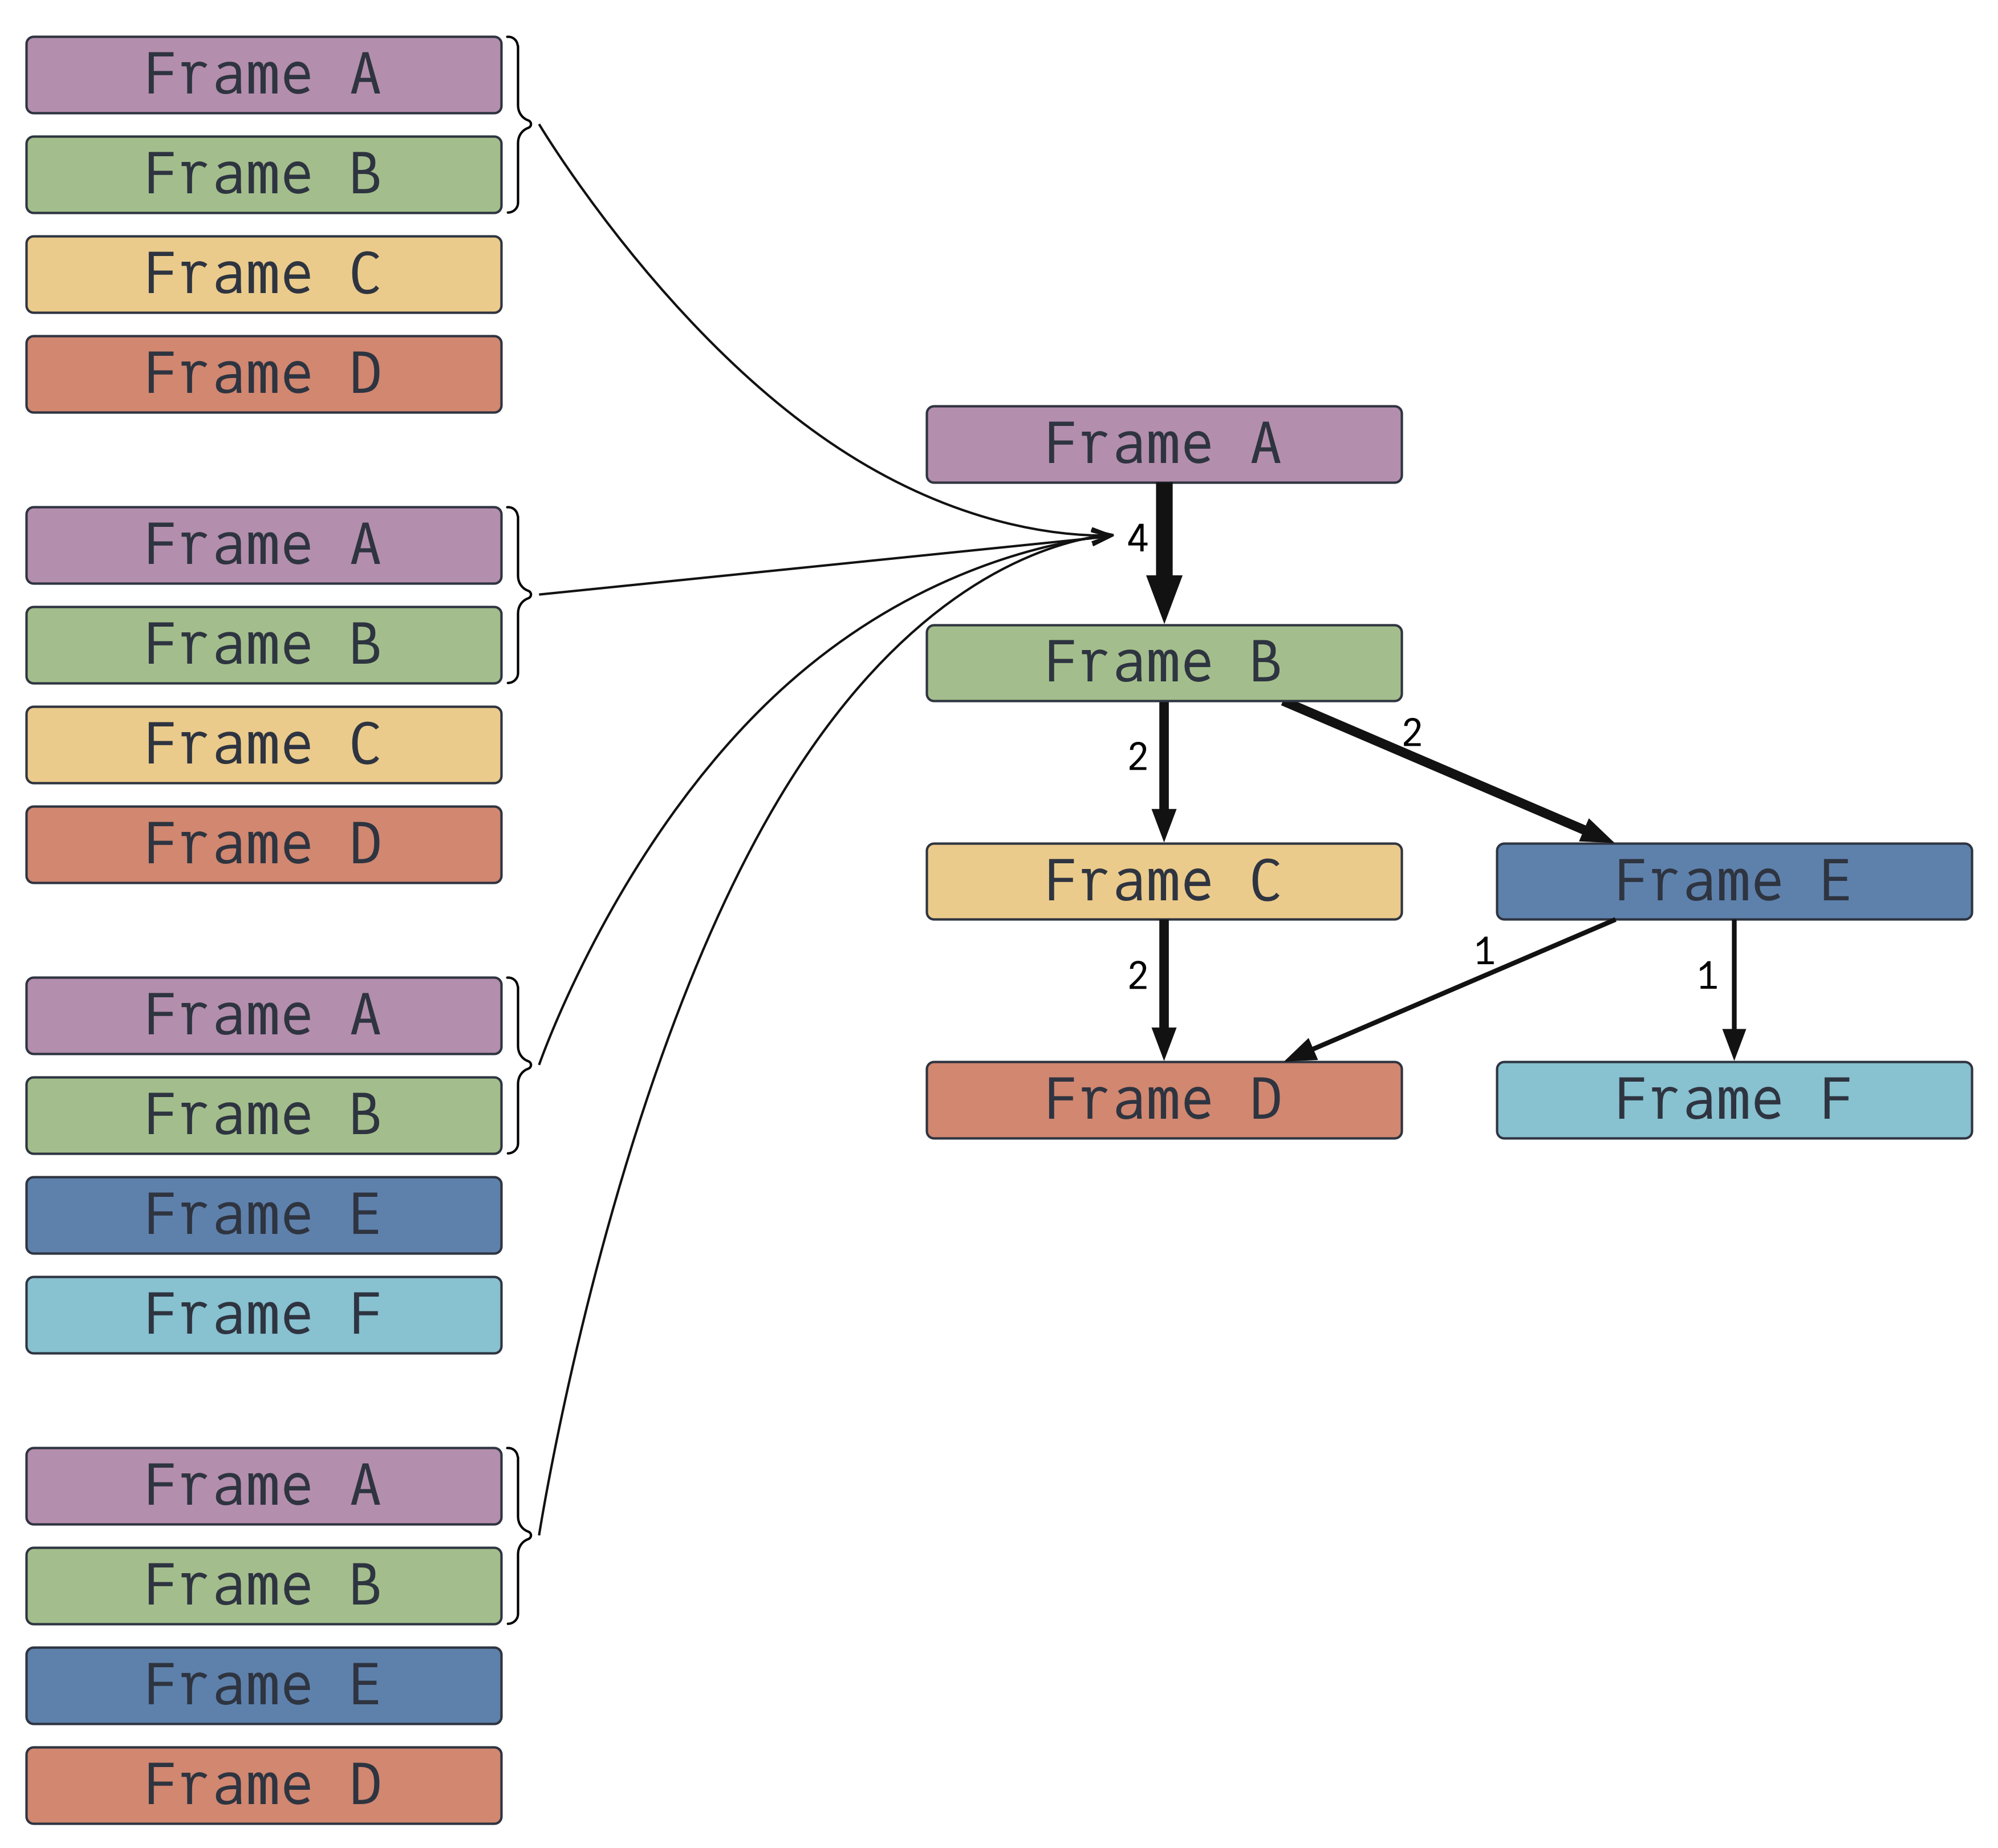
\includegraphics[width=3in]{./fig/cstg_static_diagram.png}
  \caption{CSTG makes a graph by connecting adjacent stack frames}
  \label{fig:cstg_demo}
\end{figure}

These graphs are meant to be read bottom-up: the bottom nodes are the roots where exceptional values manifested.
Higher nodes in the graph show function calls progressively closer to the top-level call that spawned them.
Thick lines and high numbers indicate flows with the highest volume leading to errors---though thin areas are still worth investigating.
CSTG provides a map to aid in contextualizing a stack trace in a log file.

\subsection{\GPUFPX{}}
\label{s:gpufpx}

% HELP: @ben, I'm not sure what paper you mean by "Julia CPU"
Many programs offload work onto GPUs, which are no less susceptible to \fp{} exceptions than CPUs.
In some regards they are \emph{more} susceptible because GPUs do not have the same exception-handling mechanisms that CPUs do.
Thus, tools to catch \fp{} exceptions on the GPU are essential.
\FT{} is constrained to CPU workloads; however, there is a companion tool called \GPUFPX{}~\cite{llsflg-hpdc-2023} that can help diagnose \fp{} exceptions on the GPU.
\GPUFPX{} can detect floating-point exceptions on the GPU that GPU code cannot do on its own.
\GPUFPX{} reports these exceptions back to the CPU for further analysis.

\FT{} and \GPUFPX{} can cover the entire computational stack, as seen in \cref{fig:ft_and_gpu_fpx}.
Work remains to tighten the integration between \FT{} and \GPUFPX{} to reduce manual work to employ both tools for heterogeneous computation.

\begin{figure}[ht]
  \centering
  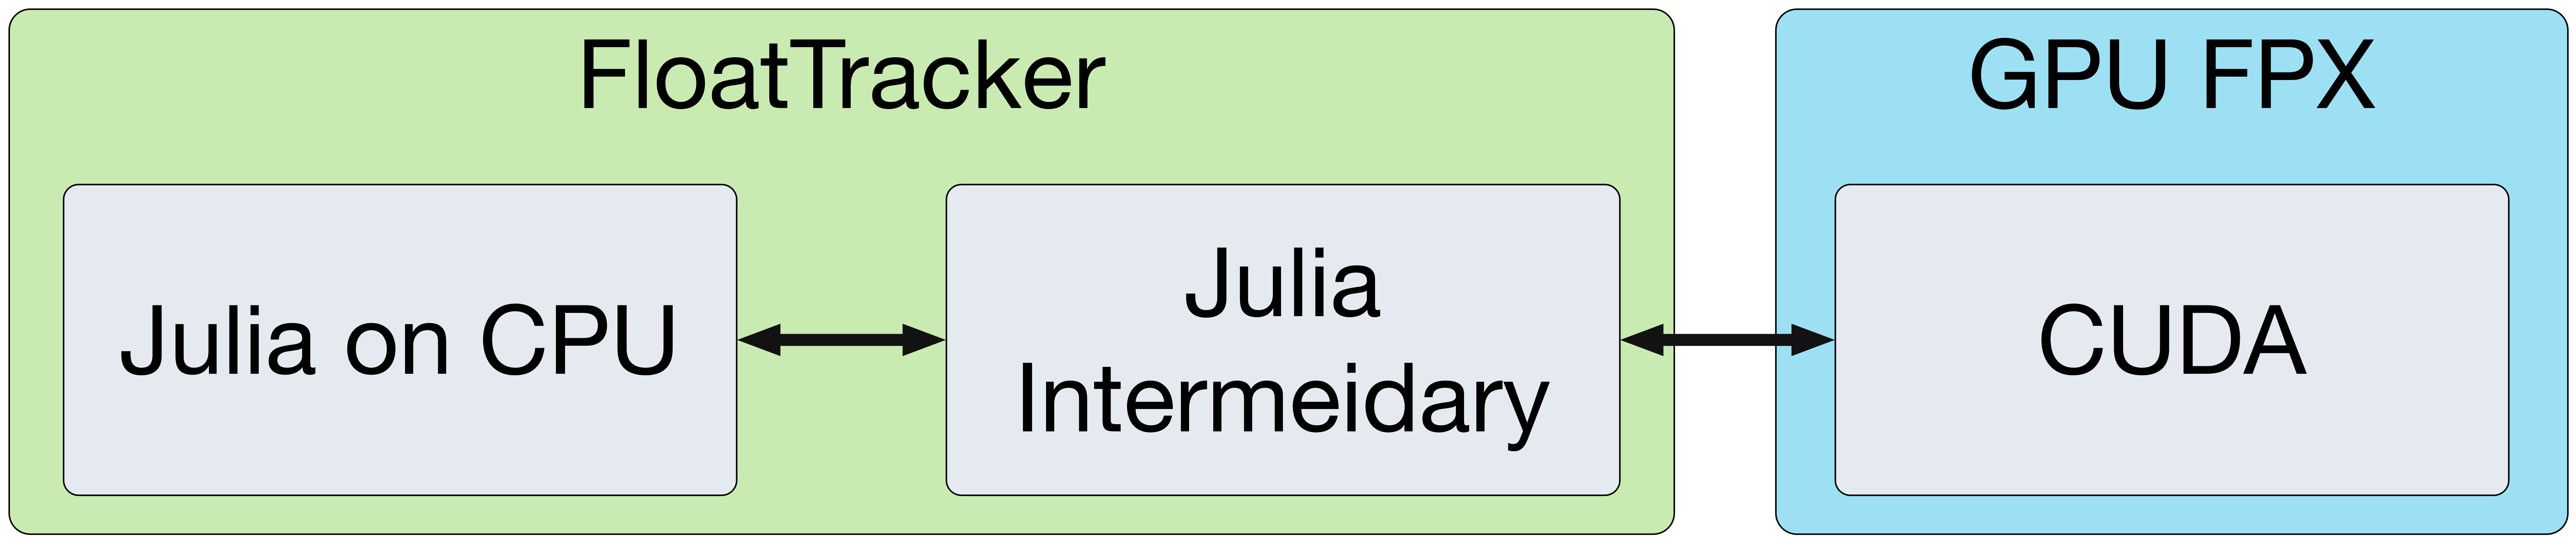
\includegraphics[width=3in]{./fig/float_tracker_context_boxes.png}
  \caption{FloatTracker and GPU-FPX compliment each other}
  \label{fig:ft_and_gpu_fpx}
\end{figure}

\section{Case Studies}
\label{s:casestudies}

In this section we'll discuss some case studies where tools from \FlowFPX{} aided in finding or fixing \fp{} issues.
\Cref{s:sw} covers an ocean simulation that produces \NaN{}s in the output---a common and frustrating occurrence for many a scientist. \Cref{s:ode} puts the popular \texttt{OrdinaryDiffEq} solver library under a fuzzer to harden it against bad behavior in the presence of exceptional \fp{} values. \Cref{s:finch} fuzzes another library---this time a library for specifying partial differential equations (PDEs). Finally, in \cref{s:ocean}, we examine another ocean simulation library---this time the library runs on the GPU. This puts it out of reach of \FT{}, but \GPUFPX{} can handle it. In addition to the case studies that we did ourselves, \cref{s:safari} is an ``in the wild'' usage of \FT{} that helped researchers uncover the source of a \NaN{} in their own code without help from us.

\subsection{ShallowWaters}
\label{s:sw}

\texttt{ShallowWaters}~\cite{klowerNumberFormatsError2020,klowerPositsAlternativeFloats2019,klowerLowprecisionClimateComputing2021} simulates the flow of water over a seabed.
This is not a general shallow waters simulation library---it is designed primarily to showcase numerical methods involving 16-bit floats.

The Courant-Friedrichs-Lewy (``CFL'') parameter roughly describes the size of the time step to take in running the simulation.
Normally this value sits between 0 and 1---smaller values mean the simulation runs slower but with higher accuracy, whereas higher values mean the simulation takes bigger time steps and consequently runs faster, but results might be inaccurate.
The primary reason for problems arising comes from information not having enough time to propagate through the simulation before the next time step is taken.

It is not uncommon to encounter cases where setting the CFL parameter too high results in \NaN{}s in the result.
Driving the CFL parameter low enough to excise the \NaN{}s can make the simulation too long and unwieldy to be comfortable to use.
Identifying where \NaN{}s begin to arise can help point the way to where some mathematical refinement can be used to make the simulation both fast and accurate enough for practical use.

We dialed the CFL parameter up to extraordinarily high values and we started seeing \NaN{}s in the result.
\code{ShallowWaters} detected the instability, but not before producing some bad output.

\begin{figure}[ht]
  \centering
  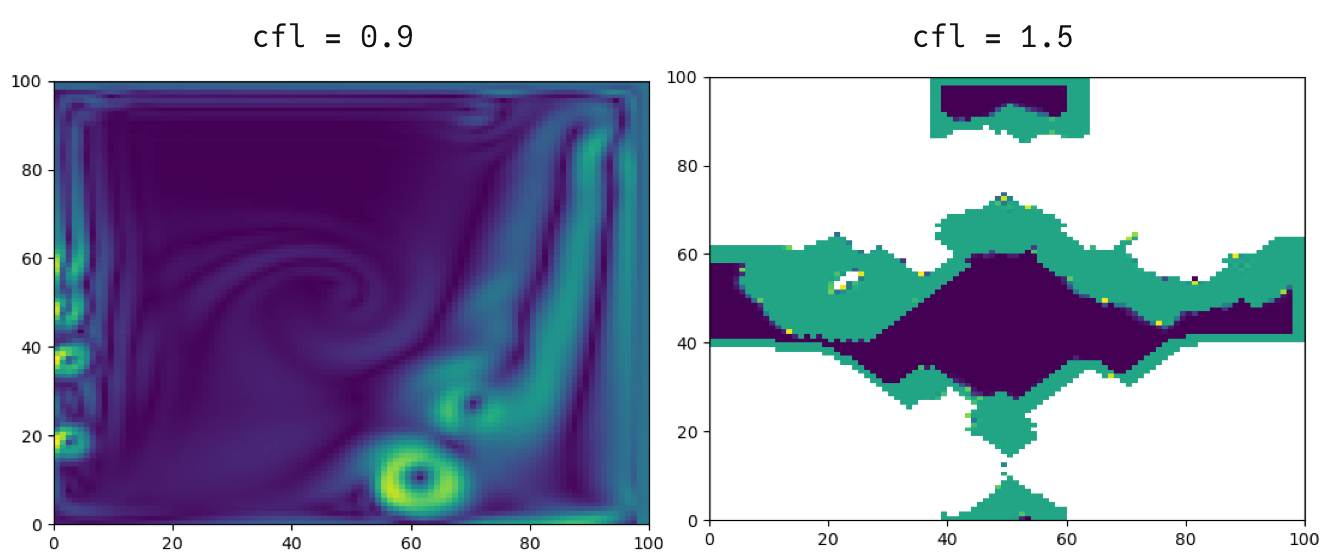
\includegraphics[width=3in]{./fig/shallow_waters_cfl_diff.png}
  \caption{Effect of high CFL parameters: on the left, normal output. On the right: \NaN{}s cause white holes and gaps in the result.}
  \label{fig:sw_nans}
\end{figure}

The white regions in the right graph of \cref{fig:sw_nans} are regions where \NaN{}s crept into the computation and destroyed the results.
In one regard, this is not as bad as a \NaN{} kill---knowing that there are \NaN{}s in the computation means that we have a chance to fix it, whereas a \NaN{} kill might silently give us the wrong answer.
Incidentally, we know that there were no \NaN{} kills in this test all the events in our kill logs are from calling the \texttt{isnan} function---a clear sign that the program is deliberately taking action on the presence of a \NaN{}.

Finding the sources of \NaN{}s can be tricky.
We expected \NaN{}s in this case because we set the CFL parameter up so high, but tracking down the sources of \NaN{}s generally is a difficult and time-consuming problem.

\FT{} solves this problem for us by automatically tracking all sources of potential \NaN{} generation.
And in this case \texttt{ShallowWaters} makes this doubly easy:
\texttt{ShallowWaters} was designed to showcase physics simulations using variable levels of \fp{} precision, and allows you to specify a \fp{} type to use in the computation.
We simply asked it to use our \texttt{TrackedFloat32} type, and then the entire simulation ran under the supervision of FloatTracker.

\begin{lstlisting}[language = Julia]
run_model(T=TrackedFloat32,
          cfl=10, Ndays=100, nx=100, L_ratio=1,
          bc="nonperiodic",
          wind_forcing_x="double_gyre",
          topography="seamount")
\end{lstlisting}

This produced almost 17000 lines of logs in the gens file. Below is a sample stack trace from these logs: (formatted for clarity)

\begin{verbatim}
-([-Inf, -Inf])   FT/TrackedFloat.jl:106
momentum_u!       ShallowWaters/rhs.jl:246
rhs_nonlinear!    ShallowWaters/rhs.jl:50
rhs!              ShallowWaters/rhs.jl:14 [inlined]
time_integration  ShallowWaters/time_integration.jl:77
run_model         ShallowWaters/run_model.jl:37
top-level
\end{verbatim}

We can see that the \NaN{} appeared as the result of $-\infty - -\infty$ (first line) and that subtraction happened in the \texttt{momentum\_u!} function on line 246 of the \texttt{rhs.jl} file (second line).
Thus, with little effort we were able to track down where the \NaN{}s were originating.

Now the question is: where did the $\infty$ come from?
We can look at the file of the $\infty$ gens where we see the following: (formatted for clarity)

\begin{verbatim}
^([-1.515f31, 2])            FT/TrackedFloat.jl:138
…
materialize(^)               broadcast.jl:860
top-level getproperty(P, :u) examples/sw_nan_tf.jl:14
…
\end{verbatim}

It looks like the $-\infty$ came from $-1.515e31^2$---no wonder a Float32 type couldn't handle something that large.
We can tell that because the first line shows us the arguments\footnote{There is a configuration option that allows us to control this behavior.} and the second line shows us what function got called.

Now we have some concrete values to work with: instead of wondering where an opaque \Inf{} or a \NaN{} came from, we have \emph{specific} values that a domain expert can use to diagnose the problem.

\subsubsection{CSTGs Help Us Get a Bigger Picture}

Running FloatTracker can produce a lot of logs.
To get a quick overview of the most common paths to problems, we can use CSTG to get an overview of what stack frames appear the most often.

\begin{figure}[ht]
  \centering
  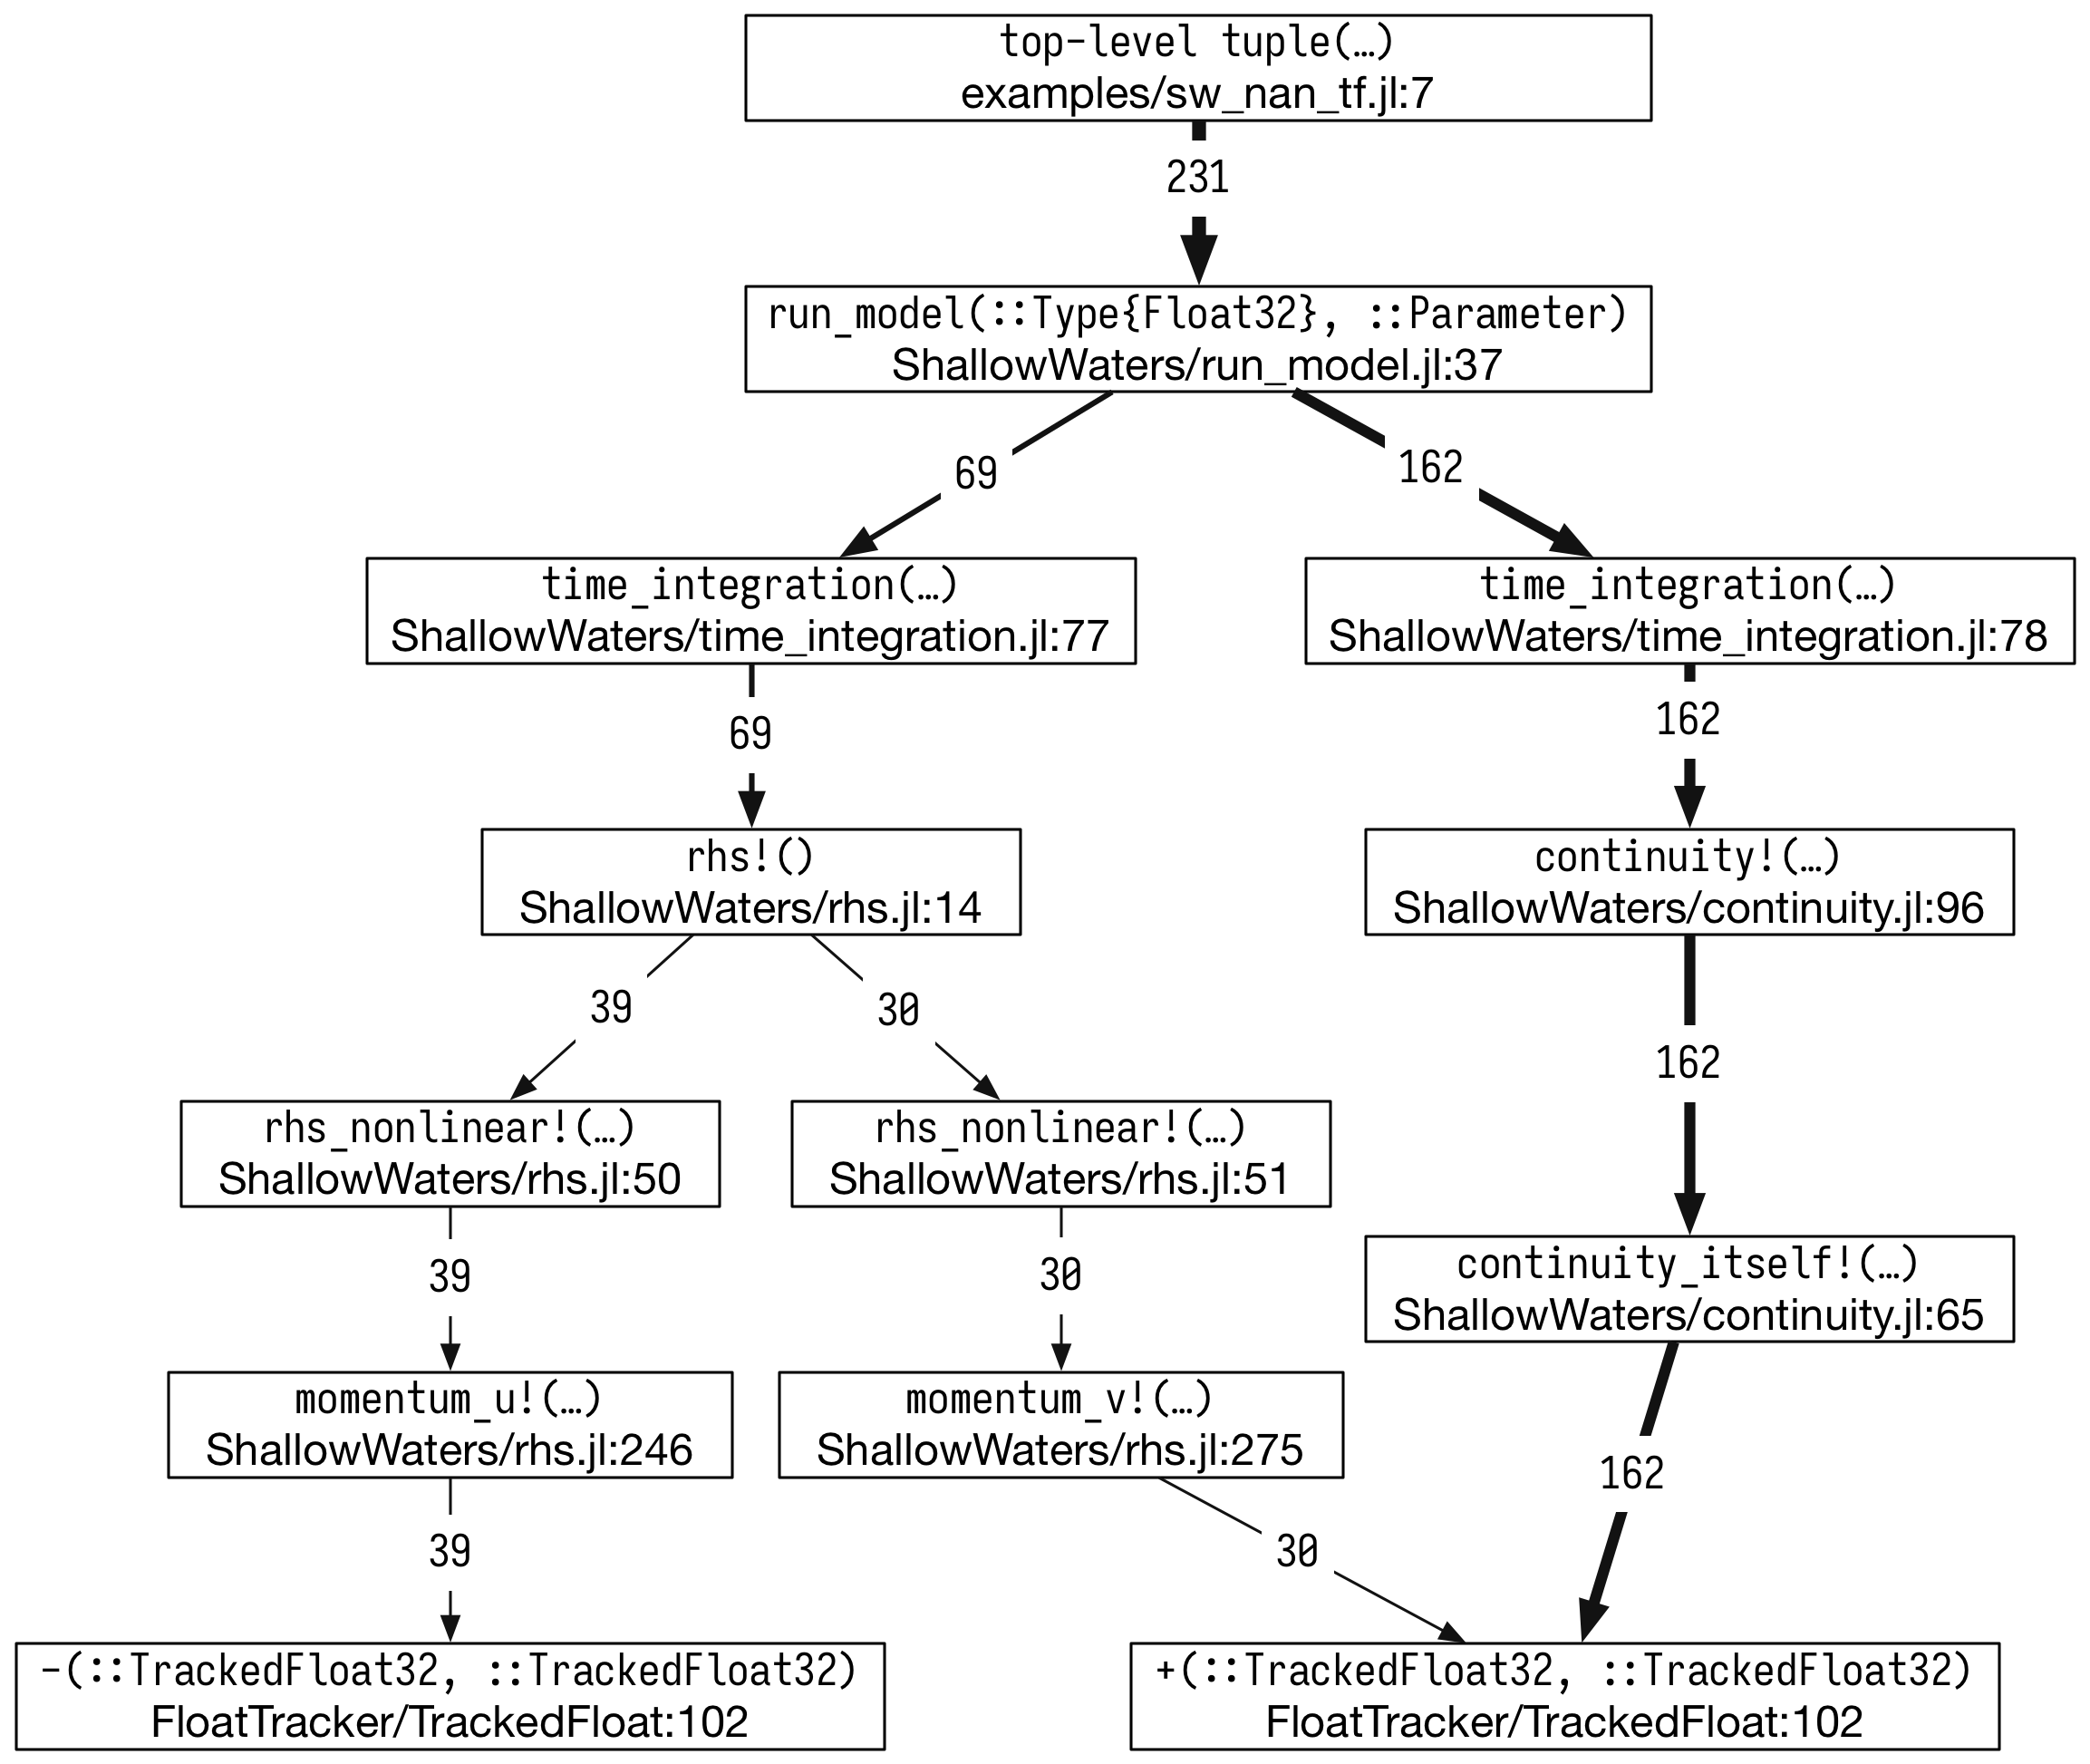
\includegraphics[width=3in]{fig/sw_nan_cstg_clean.png}
  \caption{CSTG of \NaN{} generation logs from ShallowWaters.}
  \label{fig:sw_nan_cstg}
\end{figure}

We can produce a CSTG of both the \Inf{} as well as the \NaN{} logs.
Here is what the two graphs look like:\footnote{As with the call stack logs, these have been edited for clarity. We only remove a few boxes in between—mostly due to space constraints in this paper.}

\begin{figure}[ht]
  \centering
  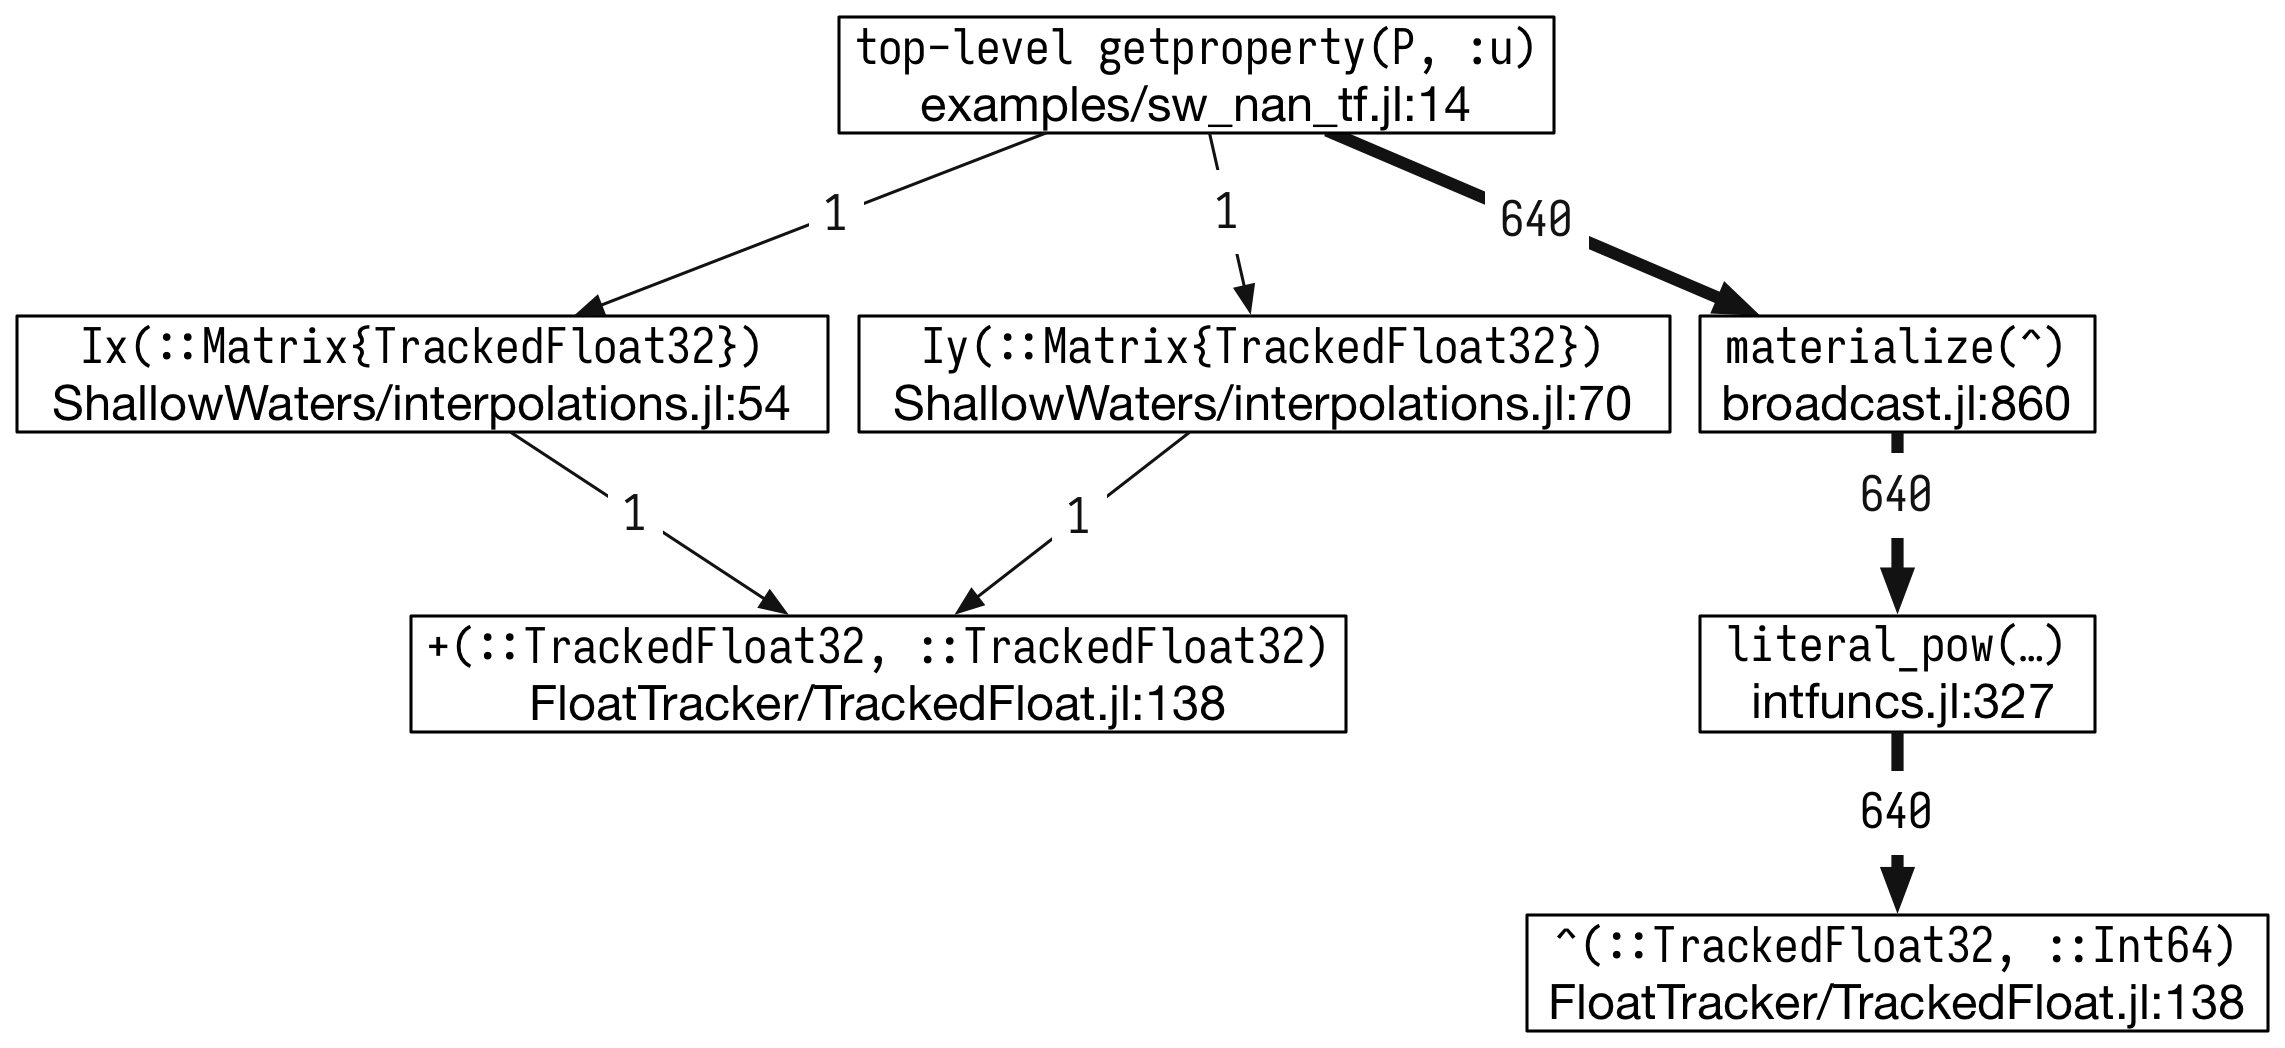
\includegraphics[width=3in]{fig/sw_inf_cstg_clean.png}
  \caption{CSTG of \Inf{} generation logs from the same run as~\cref{fig:sw_nan_cstg}.}
  \label{fig:sw_inf_cstg}
\end{figure}

Another one of CSTGs abilities is \emph{graph diffing}.
We took the \FT{} logs from running ShallowWaters and split the logs at the 10\% mark.
We used CSTG to diff the flow graphs between the first 10\% of the run of the program and the remaining 90\%.
The diff can be seen in \cref{fig:cstg_diff_demo}.

\begin{figure}
  \centering
  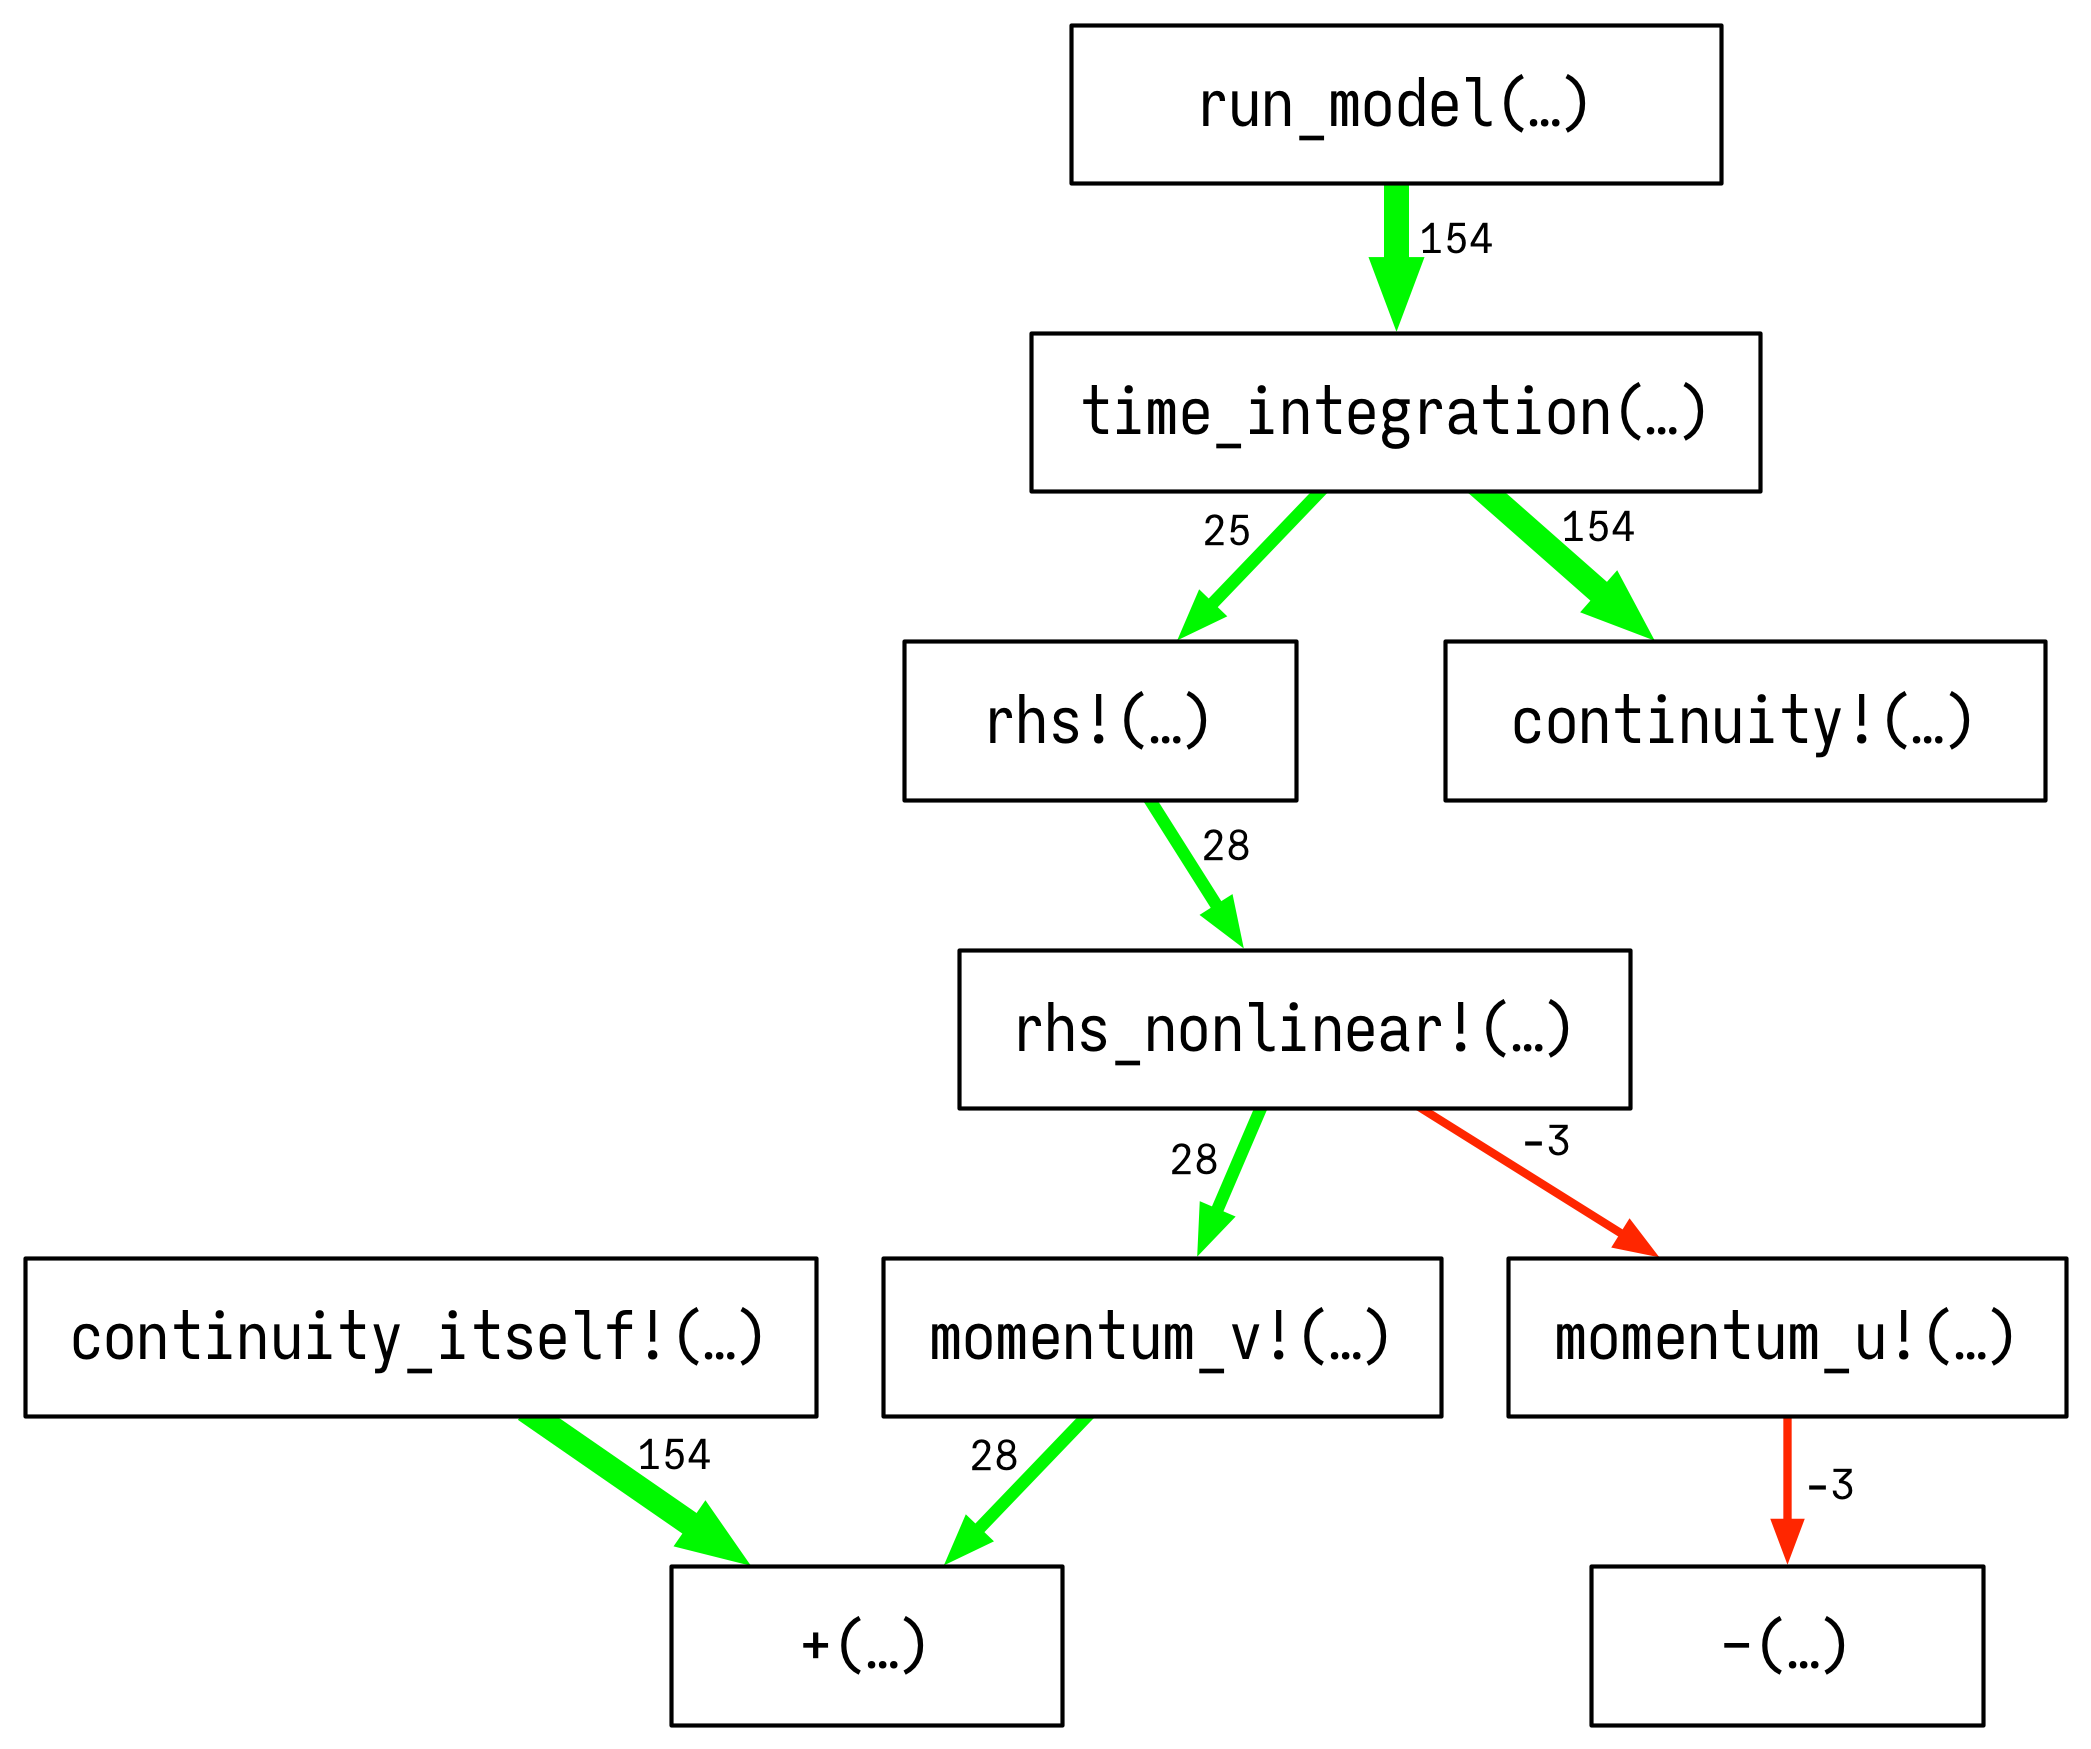
\includegraphics[width=3in]{./fig/cstg_diff_pretty.png}
  \caption{Diff between the early and latter stages of ShallowWaters}
  \label{fig:cstg_diff_demo}
\end{figure}

The green lines indicate flows that were \emph{new} in the latter 90\% of the program's run.
The red lines indicate flows that were \emph{only in} the first 10\% of the program's run.
What this means depends on the particular program; a domain expert can use these clues to e.g. find where instability started in the first part of the program, and where that instability got reinforced later on.

\subsection{OrdinaryDiffEq}
\label{s:ode}

To exercise the fuzzing abilities of \FT{}, we tried fuzzing \texttt{NBodySimulator}\footnote{\url{https://github.com/SciML/NBodySimulator.jl}} from the SciML team, which simulates the gravitational interactions between two or more massive bodies.
However, when we used \FT{}, we got no \fp{} operations.
We discovered that \texttt{NBodySimulator} merely sets up the system of equations to solve, then hands all the work of running the simulation off to the \texttt{OrdinaryDiffEq}\footnote{\url{https://github.com/SciML/OrdinaryDiffEq.jl}} library from the same team.

We configured \FT{} to inject a single \NaN{} somewhere within the scope of the \texttt{NBodySimulator} and \texttt{OrdinaryDiffEq} libraries.
We found a run where something curious happened: the library reported that it had detected a \NaN{} and would then exit.
However, after printing that message, the program went into an infinite loop.

% FIXME: should I show that CSTG here in the paper?
We used CSTGs to get an idea of what the important flows were in the run of this errant behavior.
With an idea of what was going on, we took a look at the logs and found a \NaN{} kill inside the \texttt{solve.jl} file in the \texttt{OrdinaryDiffEq} library.

\begin{verbatim}
…
<       at FloatTracker/src/TrackedFloat.jl:193
solve!  at OrdinaryDiffEq/src/solve.jl:515
…
\end{verbatim}

The relevant part of \texttt{solve.jl} looks like this:

% file here: ~/Research/ode_debug/dev/OrdinaryDiffEq/src/solve.jl
% see line 514

\begin{lstlisting}[language = Julia]
while !isempty(time_stops)
  while tdir * t < first(time_stops)
    # do integration work
    # pop_off(time_stops)
  end
end
\end{lstlisting}

The problem here is on line 2 when \texttt{tdir} is \NaN{}: multiplication propagates \NaN{}s, and comparison kills it, so the condition on the inner \texttt{while} loop is \emph{always} false.
No work got done in the inner loop, and so the size of the \texttt{time\_stops} vector never decreases.

Our kill logs led us right to this line; this is a perfect example of how \NaN{} kills can influence control flow to go awry.
In this case, the problem was apparent besides what our logs told us and it manifested as an infinite loop.
More dangerous cases can occur when the influence of a bad comparison is not as readily observable.
In any case, \FT{} can help monitor for kills and help fuzz to find kills before they arise in production.

We were able to use the injection recording and the gen logs to track down where the first \NaN{} was injected to cause the infinite loop.
This made it simple for us to create an example to reproduce the behavior, which we included in the GitHub issue that we opened.\footnote{\url{https://github.com/SciML/OrdinaryDiffEq.jl/issues/1939}}

\subsection{Finch}
\label{s:finch}

Finch is a domain-specific language for specifying
PDEs~\cite{heislerFinchDomainSpecific2022}.\footnote{Not to be confused
with the Finch loop optimizer~\cite{adka-cgo-2023}.}
In the spirit of FEniCS~\cite{fenics} and related
tools~\cite{freefem,openfoam,dune,firedrake},
Finch helps scientists quickly convert math into code.
What sets Finch apart is its flexibility.
It supports multiple discretization methods (finite element and finite
volume) and multiple backends (Julia, \CPP{}, \Dendro{}~\cite{dendro}).
Furthermore it strives to output code that humans can easily fine-tune.

Fuzzing with \FT{} revealed two places where Finch needed
protection against user input.
The first was when reading an input mesh.\footnote{\urlaccess{https://github.com/paralab/Finch/issues/16}{2023-06-06}}
A \NaN{} injected in the mesh led to a crash further on:
\begin{verbatim}
  BoundsError: attempt to access 1-element
   Vector{Int64} at index [2]
\end{verbatim}
Defensive programming solves the issue.
The second place was in setting bounds for the
solver.\footnote{\urlaccess{https://github.com/paralab/Finch/issues/17}{2023-06-06}}
Here, a \NaN{} could leave bounds uninitialized, leading to a bounds error.
Additionally, \FT{} and \CSTG{}s have been useful for identifying \NaN{}s that
appear in unstable systems.
%% advection2d, high cfl and high T (time) led to NaN during simulation

\subsection{\GPUFPX{}: Oceananigans}
\label{s:ocean}

Oceananigans~\cite{OceananigansJOSS} is simulation package for incompressible
fluid dynamics that can generate code for Nvidia GPUs.
For example, the following program (from the project readme) simulates turbulance:

\begin{lstlisting}[language = Julia]
using Oceananigans
grid = RectilinearGrid(GPU(),
  size=(128, 128), x=(0, 2π), y=(0, 2π),
  topology=(Periodic, Periodic, Flat))
model = NonhydrostaticModel(; grid,
  advection=WENO())
ϵ(x, y, z) = 2rand() - 1
set!(model, u=ϵ, v=ϵ)
simulation = Simulation(model;
  Δt=0.01, stop_time=4)
run!(simulation)
\end{lstlisting}

\GPUFPX{} provides detailed feedback on this program.
The output in~\cref{f:gpufpx} shows that 21 kernels
appear and generate six floating-point exceptions.
There are three \NaN{}s, one \Inf{}, and two division
by zero errors.
The report is a starting point for further investigation
of the reliability of the example.
%% TODO exactly how?

\begin{figure}[t]\centering
  \begin{tabular}[t]{ll}
    \begin{tabular}[t]{lr}
      \zerocode{-{}- FP64 Operations -{}-} \\
      \code{Total NaN:} & \code{2} \\
      \code{Total INF:} & \code{1} \\
      \code{Total subnormal:} & \code{0} \\
      \code{Total div0:} & \code{2} \\
    \end{tabular}
    &
    \begin{tabular}[t]{lr}
      \zerocode{-{}- FP32 Operations -{}-} \\
      \code{Total NaN:} & \code{1} \\
      \code{Total INF:} & \code{0} \\
      \code{Total subnormal:} & \code{0} \\
      \code{Total div0:} & \code{0} \\
    \end{tabular}
  \end{tabular}
  \begin{tabular}{lr}
    \zerocode{-{}- Other Stats -{}-} \\
    \code{Kernels:} & \code{21}
  \end{tabular}

  \caption{Example \GPUFPX{} output}
  \label{f:gpufpx}
\end{figure}

\subsection{RxInfer: No Help Needed}
\label{s:safari}

\FT{} has proven to be useful for more than its creators---we discovered an open issue in the \code{RxInfer.jl} library with an issue revolving around \NaN{} detection.\footnote{\url{https://github.com/biaslab/RxInfer.jl/issues/116}}
Even though we were unable to provide hands-on guidance as the code in question was proprietary, the authors of \code{RxInfer.jl} were able use \FT{} themselves, and within a day they tracked down the location of a \NaN{} gen.
The \code{RxInfer.jl} authors provided us with valuable feedback on \FT{}'s API.

\section{Related Work}
\label{s:related}

\subsection{Floating-Point Error Analysis}

Demmel et al.\cite{ddghlllprr-correctness-2022} examine \fp{} exceptional value handling in the BLAS and LAPACK libraries and propose solutions to inconsistencies.
They describe a proposal to pack numeric codes into an \texttt{INFO\_ARRAY} that mirrors our gen-prop-kill framework.
They also suggest a fuzzing technique that we realize in \FT{}:
instead of fuzzing the \emph{inputs} to a program, we fuzz by randomly injecting exceptional values at \emph{any} point where there is an arithmetic operation. Demmel suggests that this approach is useful since any \fp{} operation could lead to an exceptional value if the inputs are in dangerous ranges.

Toronto and McCarthy\cite{torontoPracticallyAccurateFloatingPoint2014} developed a methodology for assessing where arithmetic operations are liable to magnify \fp{} error.
Their work includes error visualization and work on how to avoid error-magnifying ``badlands''.
They focus on rewriting arithmetic expressions to avoid error which could lead to exceptional values, rather than on exceptional values themselves.

In a similar vein, Herbie\cite{panchekhaAutomaticallyImprovingAccuracy2015} is a tool for automatically rewriting arithmetic expressions to reduce \fp{} error.
\FT{} tracks down exceptional \fp{} values; once the location of a gen is found, Herbie could be employed to rewrite the arithmetic expression, if \fp{} error is the cause of the exceptional value.
Odyssey\cite{misbackOdysseyInteractiveWorkbench2023} provides a helpful interactive interface to the tooling that Herbie provides.

\subsection{Diagnosing floating-point exceptions}

The Julia library \texttt{Sherlogs}\footnote{\url{https://github.com/milankl/Sherlogs.jl}} by Milan Klöwer inspired the use of a custom number type to intercept operations on a number.
In contrast to \FT{} which monitors for exceptional values and logs stack traces at interesting points in their lifetime, \texttt{Sherlogs} tracks and reports the range of values seen over the course of a computation.
This is intended to provide insight into whether or not a library could tolerate a lower-precision \fp{} format.

% TODO: make sure that what I said about what FPSpy can track is true.
FPSpy~\cite{dindaSpyingFloatingPoint2020} is an \texttt{LD\_PRELOAD} shared library that works on unmodified x86 binaries.
It can monitor a program during execution for any \fp{} arithmetic issues, such as division by zero, denormalization, underflow, and overflow.
\FT{} in contrast focuses on the lifetime of exceptional values; \FT{} can notice when a \NaN{} gets killed, for instance, while that is not an event that FPSpy appears to be able to track.
FPSpy has the advantage of being lightweight enough to run on production code for certain loads.

\subsection{Stack Trace Graphs}

CSTG~\cite{humphreySystematicDebuggingMethods2014} is built on the work of and related to the STAT~\cite{arnoldStackTraceAnalysis2007} tool developed by Laurence Livermore National Laboratory.
STAT is a tool for collecting, analyzing, and visualizing stack traces from thousands of concurrent processes, and is designed to highlight anomalies quickly.
It produces visualizations similar to those of CSTG, thought CSTG offers more compact views.

\subsection{Floating-Point Exceptions on the GPU}

FPChecker~\cite{l-ase-2019} is a tool to report \fp{} exceptions occurring on the GPU.
FPChecker relies on LLVM-level instrumentation of GPU kernels, and so cannot run on the plethora of closed-source GPU kernels in usage today.

BinFPE~\cite{llg-soap-2022} is another tool in the same space;
BinFPE performs SASS-level analysis of GPU kernels, but is limited in that it is slow and does not catch errors that alter control flow.
The latter deficiency is particularly worrisome, as we have seen, silent \NaN{} kills can invalidate results without the user noticing.

\GPUFPX{}~\cite{llsflg-hpdc-2023} improves on the work of FPChecker and BinFPE by being more performant and catching a wider set of errors, including those that alter control flow.
\GPUFPX{} is a shared library that, like FPSpy uses \texttt{LD\_PRELOAD} to work on unmodified binaries.
\GPUFPX{} runs on CUDA cores from NVIDIA and reports total numbers of exceptional values.
Like \FT{}, \GPUFPX{} can catch \NaN{} gens and kills, but it does this on the GPU where \FT{} doesn't apply.
Despite these improvements, \GPUFPX{} is limited by the closed-source nature of common GPU cores, and cannot report at the rich level of source detail that \FT{} can.

Work is ongoing to use \GPUFPX{} and \FT{} in tandem.

% Error analysis, typical answer.
% Difficult.
% CITE

% % Herbie, improving accuracy automatically.
% % ParetoHerbie

% %% http://eprints.maths.manchester.ac.uk/2873/1/fami22.pdf
% %% https://drive.google.com/drive/folders/1HkgMpxi6hsqLSZj9tSnuCxnFExPPjmvx?usp=sharing
% %% https://docs.google.com/presentation/d/1ueqzb5QY9YHmtY2DfY_hpN9oufSOcXErLWsJOZQxgzo/edit?usp=sharing
% %% https://ieeexplore.ieee.org/document/8916392
% %% https://link.springer.com/chapter/10.1007/978-3-319-73721-8_24

% FPChecker, " considers CPU OpenMP and MPI codes, again using LLVM
% instrumentation"~\cite{ltlg-iiswc-2022}
% % FPChecker has a nice table of tools; some already mentioned here

% 6-8,24,25
% Arnab Das scalable yet rigorous
% Marc Daumas Certification of Bounds Expres
% David Delmas Towards an Industrial Use of
% Alexey Solovyev FPTaylor Results table
% Titolo absint

% GPU-FPX state of art, companion project~\cite{llsflg-hpdc-2023}.
% Latest in line of work.
% BinFPE exn checking, slower than GPU-FPX, 
% \cite{llg-soap-2022}.
% FPChecker, early pioneer, fpx in gpus, llvm-level instrumentation
% if compiled with Clang, but most gpus use closed NVCC compiler~\cite{l-ase-2019}.

\section{Discussion}
\label{s:discussion}
% future work

\subsection{Performance}
\label{s:discussion-performance}

% TODO: citations!!!!
% TODO: real numbers!!!
\FT{} incurs significant overhead on the order of 100x slower than a non-instrumented run of the same program.
To put this number into context, Valgrind runs with a similar level of slowdown.

In addition to the cost incurred by intercepting \fp{} operations, gathering stack traces is expensive---we measured a significant slowdown on the order of 10x relative to a non-logging setup of \FT{}.
We recommend that users of \FT{} make use of the \texttt{maxLogs} and \texttt{exclude\_stacktrace} configuration options to limit the number and kind of logs gathered, and thereby reduce the number of calls to \texttt{stacktrace()}.

When injection is turned on we defer the stack checks as late as we can.
Once the fuzzer runs out of \NaN{}s, it effectively turns off, so the rest of the fuzzing session proceeds much more quickly.
That said, gathering stack traces still incurs a heavy overhead during logging when interesting events occur;
we recommend limiting the number and kinds of events logged for optimal performance.

\subsection{Tracking More than \NaN{}s and \Inf{}s}

FloatTracker is capable of monitoring all sorts of events in a \fp{} value's lifetime---not just a value going to \NaN{} or \Inf{}.
We spent most of the time engineering and testing \NaN{} tracking and injection.
Adding \Inf{} tracking took a few hours.
Adding other values of interest presents no fundamental difficulties.

\subsection{Enhanced Fuzzing}

While fuzzing is useful for discovering issues, its success rate
is low because \emph{every} \fp{} operation is a candidate
for injection.
Even operations that are already well-defended against \NaN{}s are candidates.
\FT{} could use two sorts of tools for improving injection.
First, fine-grained control to let users decide where not to inject.
Second, tools for understanding the context of an injection point
after the fact.
Program slicing is especially relevant to the latter point (and effectively
what we did by hand when fuzzing Finch~\cref{s:finch}).
For each operation, an expert needs to study the values that feed into it to
decide whether they are protected or not.

%% TODO example, start here at glbvertex https://github.com/paralab/Finch/blob/master/src/grid.jl#L360

\subsection{Tracking Exceptions in External Libraries}

\FT{}'s scope is limited to Julia code: it cannot track the lifetime of exceptional values that are born, live, or die in external libraries, such as C programs.
One approach would be to create an API for \FT{} so that programs using these external libraries could leverage \FT{}'s tooling to monitor the interface between Julia and e.g. external C programs.

\subsection{Future Work}

\FlowFPX{} is a growing project and we welcome feedback from domain experts
on how to best suit their workflow.
If you try any of our tools, please send us comments, suggestions, and bug reports via the tools' repositories on GitHub.

\section{Acknowledgments}

We would like to thank Alex Larsen and Rob Durst for their help with reading drafts of the paper and feedback on the presentation.
We would also like to thank the developers of \code{RxInfer.jl} for feedback on \FlowFPX{}.
Finally, many thanks to Milan Klöwer, the author of the \texttt{Sherlogs} library, for inspiration on the architecture of \FT{}.

% **************GENERATED FILE, DO NOT EDIT**************

\bibliographystyle{juliacon}
\bibliography{ref.bib}


\end{document}

% Below is some Emacs-specific stuff to help me (Ashton) write this paper. If
% you're using Emacs, you should try using the new jinx package for
% spell-checking!

% Local Variables:
% jinx-local-words: "BinFPE CFL CSTG's CSTGs Courant Demmel FPChecker Friedrichs Herbie JuliaHub Klöwer Lewy OrdinaryDiffEq RxInfer ShallowWaters Sherlogs TrackedFloat isnan"
% citar-bibliography: ("./ref.bib")
% End:
